\begin{figure}[h!]
\begin{center}
\includegraphics[width=8cm,keepaspectratio,angle=270]{02_localization/images/7Z-frz-1.eps}
\caption{\footnotesize CAS+S energy curves (Hartree) for the cis-trans rigid
interconversion of the (7Z)-13 ammoniotridec-7-enoate with different 
cut strategies and frz-1 freeze strategy. The reference (solid black line)
is evaluated on the complete molecular system with no frozen orbitals except
the $1s$ core orbital for heavy atoms. frz-1/nocut curve (dotted line,
$\Box$ symbol) and frz-1/cut-5 (short dash line, $\times$ symbol) appear as
superposed on the drawing scale. The other curves are frz-1/cut-3 (long
dash line, $\bigcirc$ symbol) and frz-1/cut-1 (dot-dash line, $\Diamond$
symbol).  }
\label{fig:7Z-frz-1}
\end{center}
\end{figure}

